\documentclass[a4paper,12pt]{article}
%%%%%%%%%%%%%%%%%%%%%%%%%%%%%%%%%%%%%%%%%%%%%%%%%%%%%%%%%%%%%%%%%%%%%%%%%%%%%%%%%%%%%%%%%%%%%%%%%%%%%%%%%%%%%%%%%%%%%%%%%%%%%%%%%%%%%%%%%%%%%%%%%%%%%%%%%%%%%%%%%%%%%%%%%%%%%%%%%%%%%%%%%%%%%%%%%%%%%%%%%%%%%%%%%%%%%%%%%%%%%%%%%%%%%%%%%%%%%%%%%%%%%%%%%%%%
\usepackage{eurosym}
\usepackage{vmargin}
\usepackage{amsmath}
\usepackage{graphics}
\usepackage{epsfig}
\usepackage{framed}
\usepackage{subfigure}
\usepackage{fancyhdr}

\setcounter{MaxMatrixCols}{10}
%TCIDATA{OutputFilter=LATEX.DLL}
%TCIDATA{Version=5.00.0.2570}
%TCIDATA{<META NAME="SaveForMode"CONTENT="1">}
%TCIDATA{LastRevised=Wednesday, February 23, 201113:24:34}
%TCIDATA{<META NAME="GraphicsSave" CONTENT="32">}
%TCIDATA{Language=American English}

\pagestyle{fancy}
\setmarginsrb{20mm}{0mm}{20mm}{25mm}{12mm}{11mm}{0mm}{11mm}
\lhead{MA4128} \rhead{Kevin O'Brien} \chead{Week 9} %\input{tcilatex}

%http://www.electronics.dit.ie/staff/ysemenova/Opto2/CO_IntroLab.pdf
\begin{document}

\tableofcontents
\newpage
\section{Logistic Regression}
Logistic regression determines the impact of multiple independent variables
presented simultaneously to predict membership of one or other of the two
dependent variable categories.

\subsection{The purpose of logistic regression}
The crucial limitation of linear regression is that it cannot deal with Dependent Variables�s that are \textbf{\textit{dichotomous}} and categorical. Many interesting variables in the business world are dichotomous: for
example, consumers make a decision to buy or not buy (\textit{\textbf{Buy/Don't Buy}}), a product may pass or fail quality control (\textit{\textbf{Pass/Fail}}), there are good or poor credit risks (\textit{\textbf{Good/Poor}}), an employee may be promoted or not (\textit{\textbf{Promote/Don't Promote}}).


A range of regression techniques have been developed for analysing data with categorical dependent
variables, including logistic regression and discriminant analysis (Hence referred to as DA, which is the next section of course).

Logistical regression is regularly used rather than discriminant analysis when there are only two categories
for the dependent variable. Logistic regression is also easier to use with SPSS than DA when
there is a mixture of numerical and categorical Independent Variables�s, because it includes procedures for
generating the necessary dummy variables automatically, requires fewer assumptions, and
is more statistically robust. DA strictly requires the continuous independent variables  (though dummy variables can be used as in multiple regression). Thus, in instances where
the independent variables are categorical, or a mix of continuous and categorical, and the
DV is categorical, logistic regression is necessary.

\subsection{Use of Binomial Probability Theory}
Since the dependent variable is dichotomous we cannot predict a numerical value for it
using logistic regression, so the usual regression least squares deviations criteria for best fit
approach of minimizing error around the line of best fit is inappropriate.

Instead, logistic regression employs binomial probability theory in which there are only two values to
predict: that probability (p) is 1 rather than 0, i.e. the event/person belongs to one group
rather than the other. Logistic regression forms a best fitting equation or function using the
maximum likelihood method (not part of course), which maximizes the probability of classifying the observed
data into the appropriate category given the regression coefficients.

\subsection{Variable Selection}
Like ordinary regression, logistic regression provides a coefficient \textbf{b} estimates, which measures
each IV�s partial contribution to variations in the response variables. The goal is to correctly predict
the category of outcome for individual cases using the most parsimonious model.

To accomplish this goal, a model (i.e. an equation) is created that includes all predictor variables that are useful in predicting the response variable. Variables can, if necessary, be entered into the model in the order specified by the researcher in a stepwise fashion like regression.

There are two main uses of logistic regression:
\begin{itemize}
\item The first is the prediction of group membership. Since logistic regression calculates the
probability of success over the probability of failure, the results of the analysis are in
the form of an \textbf{odds ratio}.
\item Logistic regression also provides knowledge of the relationships and strengths among
the variables (e.g. playing golf with the boss puts you at a higher probability for job
promotion than undertaking five hours unpaid overtime each week).
\end{itemize}

\subsection{Assumptions of logistic regression}
\begin{itemize}
\item Logistic regression does not assume a linear relationship between the dependent and
independent variables.
\item The dependent variable must be a dichotomy (2 categories).
(Remark: Dichotomous refers to two outcomes. Multichotomous refers to more than two outcomes).
\item The independent variables need not be interval, nor normally distributed, nor linearly
related, nor of equal variance within each group.
\item The categories (groups) must be mutually exclusive and exhaustive; a case can only be
in one group and every case must be a member of one of the groups.
\item Larger samples are needed than for linear regression because maximum likelihood
coefficients are large sample estimates. A minimum of 50 cases per predictor is
recommended.
\end{itemize}

\subsection{Odds and Odds Ratio}
Logistic regression calculates changes in the log odds of the dependent,
not changes in the dependent value as OLS regression does. For a dichotomous variable the
odds of membership of the target group are equal to the probability of membership in the
target group divided by the probability of membership in the other group. Odds value can
range from 0 to infinity and tell you how much more likely it is that an observation is a
member of the target group rather than a member of the other group. If the probability is
0.80, the odds are 4 to 1 or 0.80/0.20; if the probability is 0.25, the odds are .33 (0.25/0.75).

If the probability of membership in the target group is 0.50, the odds are 1 to 1 (0.50/0.50), as
in coin tossing when both outcomes are equally likely.

Another important concept is the odds ratio (OR), which estimates the change in the
odds of membership in the target group for a one unit increase in the predictor. It is calculated by using the regression coefficient of the predictor as the exponent. Suppose we were predicting exam success by a maths competency
predictor with an estimate b = 2.69. Thus the odds ratio is exp(2.69) or 14.73. Therefore the odds of passing
are 14.73 times greater for a student, for example, who had a pre-test score of 5, than for a
student whose pre-test score was 4.
%--------------------------------------------------------%
\subsection{The Sigmoid Graph}
While logistic regression gives each predictor (IV) a coefficient \textbf{b} which measures its
independent contribution to variations in the dependent variable, the dependent variable
can only take on one of the two values: 0 or 1.

What we want to predict from a knowledge of relevant independent variables and coefficients is therefore not a numerical value of a
dependent variable as in linear regression, but rather the probability (p) that it is 1 rather
than 0 (belonging to one group rather than the other). But even to use probability as the dependent variable is unsound, mainly because numerical predictors may be unlimited in range. If we expressed p as a linear function of investment, we might then find ourselves predicting that p is greater than 1 (which cannot be true, as
probabilities can only take values between 0 and 1). Additionally, because logistic regression
has only two y values � in the category or not in the category � a straight line best fit (as in
linear regression) is not possible to draw.
\subsubsection{Hypothetical Example}
Consider the following hypothetical example:
200 accountancy first year students are graded on a pass-fail dichotomy on the end of the
semester accountancy exam. At the start of the course, they all took a maths pre-test with
results reported in interval data ranging from 0�50 � the higher the pretest score the more
competency in maths. Logistic regression is applied to determine the relationship between
maths pretest score (IV or predictor) and whether a student passed the course (DV). Students
who passed the accountancy course are coded 1 while those who failed are coded 0.
\begin{center}
\begin{figure}
  % Requires \usepackage{graphicx}
  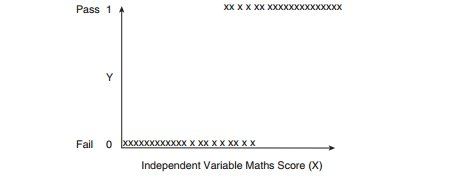
\includegraphics[scale=0.8]{Logistic1}\\
  \caption{Accountancy Exam Results}
\end{figure}
\end{center}

We can see from Figure 1 of the plotted �x�s� that there is somewhat greater likelihood
that those who obtained above average to high score on the maths test passed the accountancy course, while below average to low scorers tended to fail. There is also an overlap in
the middle area. But if we tried to draw a straight (best fitting) line, as with linear regression,
it just would not work, as intersections of the maths results and pass/fail accountancy results
form two lines of x�s, as in Figure 1.
%
%\begin{figure}
%  % Requires \usepackage{graphicx}
%  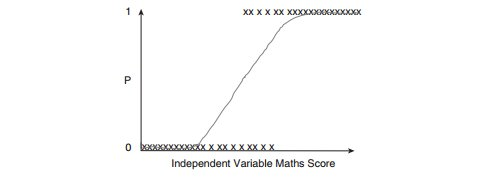
\includegraphics[width=0.40]{Logistic2.jpeg}\\
%  \caption{Figure 2}
%\end{figure}
\begin{center}
\begin{figure}
  % Requires \usepackage{graphicx}
  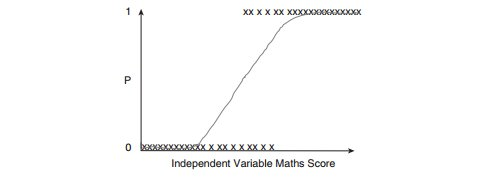
\includegraphics[scale=0.8]{Logistic2}\\
  \caption{Accountancy Exam Results - Fitted Curve}
\end{figure}
\end{center}

The solution is to convert or transform these results into probabilities. We might compute
the average of the Y values at each point on the X axis. We could then plot the probabilities
of Y at each value of X and it would look something like the wavy graph line superimposed
on the original data in Figure 2. This is a smoother curve, and it is easy to see that the
probability of passing the accountancy course (Y axis) increases as values of X increase.
What we have just done is transform the scores so that the curve now fits a cumulative
probability curve, i.e. adding each new probability to the existing total. As you can see, this
curve is not a straight line; it is more of an s-shaped curve (A sigmoid curve).

Predicted values are interpreted as probabilities and are now not just two conditions with a value of either 0 or 1 but continuous data that can take any value from 0 to 1.
The slope of the curve in Figure 2 is low at the lower and upper extremes of the
independent variable and greatest in the middle where it is most sensitive. In the middle, of
course, are a number of cases that are out of order, in the sense that there is an overlap with
average maths scores in both accountancy pass and fail categories, while at the extremes are
cases which are almost universally allocated to their correct group. The outcome is not a prediction of a Y value, as in linear regression, but a probability of belonging to one of two conditions
of Y, which can take on any value between 0 and 1 rather than just 0 and 1 in Figure 1.

\subsubsection{Log transformation}
Unfortunately a further mathematical transformation � a log transformation � is needed
to normalize the distribution. Transformations, such as log transformations and
square root transformations transform non-normal/skewed distributions closer to normality.

This log transformation of the p values to a log distribution enables us to create a link with the normal regression equation. The log distribution (or logistic transformation of p) is also called the logit of p or \textbf{\textit{logit(p)}}.

\subsection{The Logit}
The convention for binomial logistic regression is to code the
dependent class of greatest interest as 1 and the other class as 0, because the coding will
affect the odds ratios and slope estimates.

The logit(p) is the log (to base e) of the odds ratio or likelihood ratio that the dependent
variable is 1. In symbols it is defined as:
\[ logit(p) = ln \left(\frac{p}{(1-p)}\right) \]

Whereas p can only range from 0 to 1, logit(p) scale ranges from negative infinity to positive
infinity and is symmetrical around the logit of 0.5 (which is zero)

\subsection{The Logistic Regression Equation}
The form of the logistic regression equation is:
\[ logit[p(x)] =  log \frac{p(x)}{1-p(x)}  = b_0 + b_1x_1 + b_2x_2 + b_3x_3 + \ldots \]

This looks just like a linear regression and although logistic regression finds a �best
fitting� equation, just as linear regression does, the principles on which it does so are
rather different. Instead of using a least-squared deviations criterion for the best fit, it
uses a maximum likelihood method, which maximizes the probability of getting the
observed results given the fitted regression coefficients. A consequence of this is that the
goodness of fit and overall significance statistics used in logistic regression are different
from those used in linear regression.

The probability that a case is in a particular category,p, can be calculated with the following formula (which is simply another rearrangement of the previous formula).

\[p = \frac{exp(b_0 + b_1x_1 + b_2x_2 + b_3x_3 + \ldots)}{1 + exp(b_0 + b_1x_1 + b_2x_2 + b_3x_3 + \ldots)}\]

\newpage
\subsection{Exercise Data Set}
The exercise data set comes from a survey of home owners
conducted by an electricity company about an offer of roof solar panels with a 50\% subsidy
from the state government as part of the state�s environmental policy. The variables involve
household income measured in units of a thousand dollars, age, monthly mortgage, size of
family household, and as the dependent variable, whether the householder would take or decline the offer.
The purpose of the exercise is to conduct a logistic regression to determine whether family
size and monthly mortgage will predict taking or declining the offer.

For the first demonstration, we will use `family size� and
`mortgage� only. For the options, select Classification Plots, Hosmer-Lemeshow Goodness
Of Fit, Casewise Listing Of Residuals and select Outliers Outside 2sd. Retain default
entries for probability of stepwise, classification cutoff and maximum iterations.

\begin{figure}[h!]
\begin{center}
  % Requires \usepackage{graphicx}
  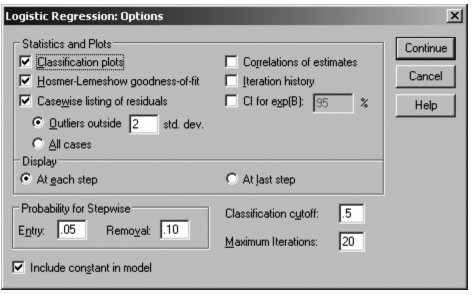
\includegraphics[scale=0.8]{Logistic10}\\
  \caption{Selected Options for Exercises}
\end{center}
\end{figure}

We are not using any categorical variables this time. If there are categorical variables, use the \textbf{\textit{categorical}} option. For most situations, choose the �indicator� coding scheme (it is the
default).


UseR! 2013 Conference

Flights to Madrid

Venue UCLM

Registration date

Abstracts

2011 Conference

Tutorials

LondonR Conference
London - R in Insurance conference
